\section{Coordinate Transformations}
\label{coordinate_transformations}


In order to  track how a rigid body such as a seld-driving car moves, we need to know how we can express its motion using
mathematical tools and notation. In this section, we will review how reference frames affect vector coordinates, compare and contrast different
rotation representations, and present several reference frames.


\subsection{Vectors}

Generally, kinematic variables, such as the velocity, are represented in the form of a vector, with both magnitude and direction. In Figure \ref{vector_rotation}, the vector $v$ is presented with a green arrow in a two-dimensional coordinate frame. We have two coordinate frames displayed here. The body frame, defined by axes $b_1$ and $b_2$, and the inertial frame defined by axes $e_1$ and $e_2$, both in the 2D plane.


\begin{figure}[!htb]
\begin{center}
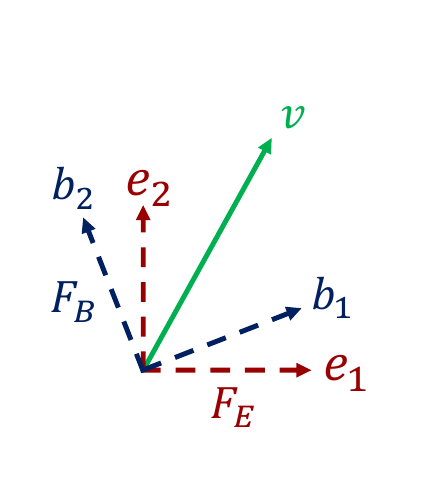
\includegraphics[scale=0.290]{img/coordinate_transforms/vector_rotation.jpeg}
\end{center}
\caption{Schematic of vector rotation in 2D.}
\label{vector_rotation}
\end{figure} 

By definition a vector  is a geometric object that has a magnitude and a direction.
Often, we treat the concept of a vector interchangeably with the concept
of vector coordinates, or the set of numbers that represent the direction and maginitude of the vector. This, however, is not necessarily correct. 
If we imagine that the vector is fixed in space, then its coordinates will change depending on the way in
which we observe it. More precisely, the same
vector quantity will have different coordinates depending on which coordinate
frame or reference frame we choose to express it in.

\begin{framed}
\theoremstyle{remark}
\begin{remark}{\textbf{Notation}}

Let us introduce some notation that will be useful susequently. 
In frame $a$, the vector $\mathbf{r}$ has notation $\mathbf{r}_a$. Likewise in frame $b$, it has the coordinates $\mathbf{r}_b$. 
The coordinates of the vector in the two different frames are related through a rotation matrix $\mathbf{C}_{ba}$

\begin{equation}
\mathbf{r}_b = \mathbf{C}_{ba}\mathbf{r}_a
\end{equation}

The rotation matrix tells us exactly how one frame is rotated with respect to the other.
\end{remark}
\end{framed} 


\subsection{2D rotations}

Let us first discuss two dimensional rotations. Assume the two coordinate frames; frame $e$ and frame $b$, which have the same fixed origin. 
Frame $b$ is rotated by some angle $\theta$ relative to frame $e$. We can then define the rotational matrices $C_{eb}$, which transforms vectors from the frame $b$ to the frame $e$ and $C_{be}$ which projects the frame $e$ onto frame $b$ using the angle $\theta$ as shown.

\begin{equation}
C_{EB} = 
\begin{bmatrix}
 \cos(\theta) & \sin(\theta) \\
 -\sin(\theta) & \cos(\theta) 
\end{bmatrix}, ~~
C_{BE} =
\begin{bmatrix}
 \cos(\theta) & -\sin(\theta) \\
 \sin(\theta) & \cos(\theta)
\end{bmatrix} 
\end{equation}

\begin{figure}[!htb]
\begin{center}
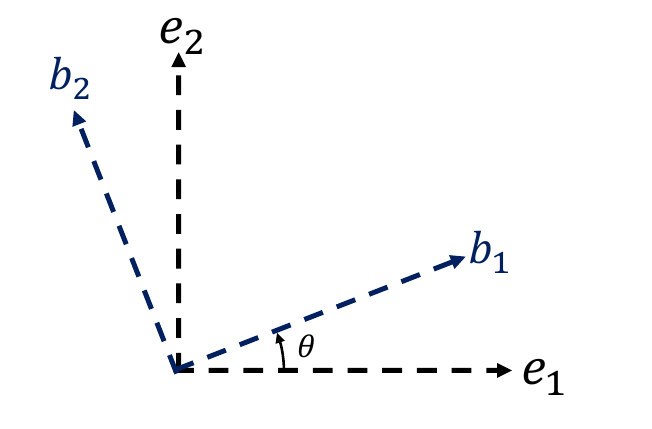
\includegraphics[scale=0.290]{img/coordinate_transforms/theta_angle.jpeg}
\end{center}
\caption{Rotation angle $\theta$.}
\label{theta_angle}
\end{figure}


Now, let's extend our example to include a translation. Here, we see a two-wheeled robot and we'd like to represent the position of a point $P$ 
observed by the robot in the robot body frame $b$, with respect to the inertial frame $e$. 
The position of the robot with respect to the inertial frame is $(x, y)$, and the orientation of the robot once again is $\theta$.


\begin{figure}[!htb]
\begin{center}
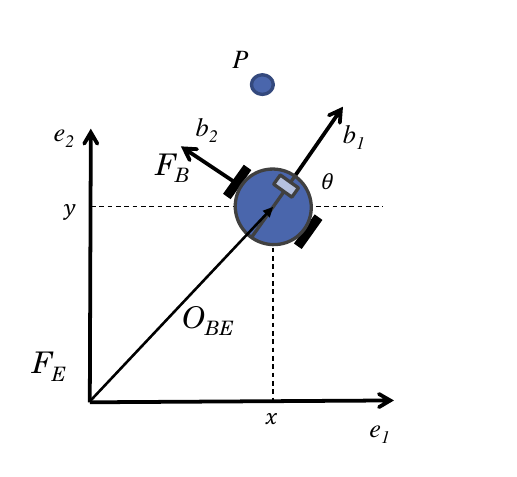
\includegraphics[scale=0.290]{img/coordinate_transforms/robot_orientation.jpeg}
\end{center}
\caption{Robot rotation and translation.}
\label{robot_orientation}
\end{figure}

The following equations relate the location of point $P$ in the body coordinates $P_b$ and the inertial frame $P_e$. 
Note that in general to transform one point from one coordinate to the other coordinate frame, body to inertial and vice versa, requires two terms. The translation of the origin $O_{be}$ and $O_{eb}$ in this case, and the rotation of the axis $C_{eb}$ and $C_{be}$. Finally, we can summarize the transformation between two coordinate frames using homogeneous coordinates, which lead to a compact matrix multiplication to apply the transformation. 

\begin{equation}
P_b = C_{eb}(\theta)P_e + O_{eb}
\end{equation}

where $O_{eb}$ is the translation term expressed in body frame. Similarly,

\begin{equation}
P_e = C_{be}(\theta)P_b + O_{be}
\end{equation}


%We extend our location vector to include $(x, y)$, and one and can then transform from body to inertial coordinates using $P$ inertial is $C_{eb}$ and $O_{eb}$ times $P$ in the body frame. 




Often, it will also be useful to know how the coordinates of points change as we move from
one reference frame to another. For example, we may know the position
of a building in some frame, and now we would like to know its position in our current vehicle frame. 
To compute this, we use vector addition making sure to express all of the
coordinates in the same reference frame. We will use superscripts on the coordinates to indicate the start and
end point of a 3D vector, again from right to left, and a subscript to indicate
the frame in which this is expressed just as before. We can manipulate this expression
to solve for the coordinates in the vehicle frame or an appropriate
inertial frame, for example, see Figure \ref{coordinate_rotations_2}.

\begin{figure}[!htb]
\begin{center}
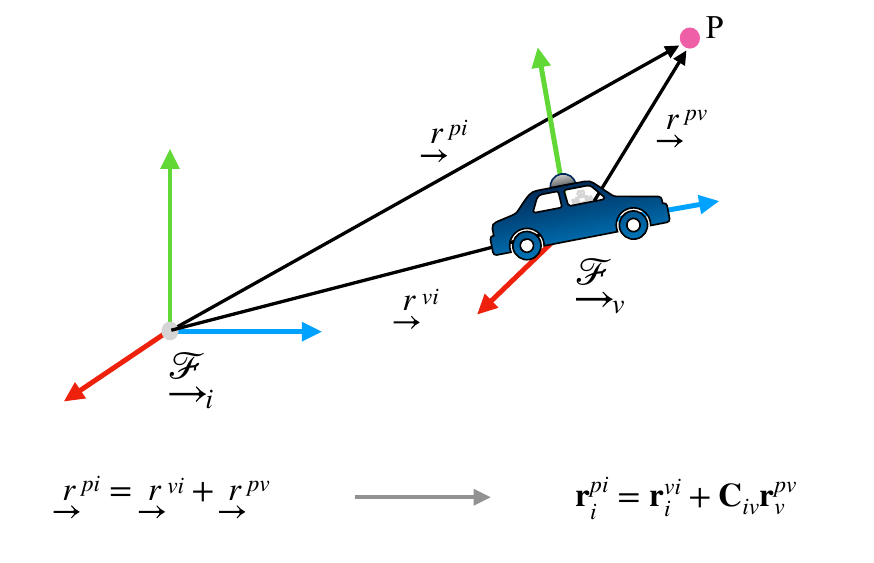
\includegraphics[scale=0.290]{img/coordinate_transforms/coordinate_rotations_2.jpeg}
\end{center}
\caption{Schematic of coordinate frames.}
\label{coordinate_rotations_2}
\end{figure}


%\begin{figure}[!htb]
%\begin{center}
%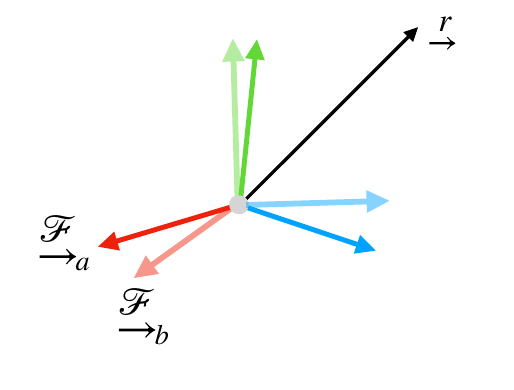
\includegraphics[scale=0.290]{img/coordinate_transforms/coordinate_rotations_1.jpeg}
%\end{center}
%\caption{Schematic of coordinate frames.}
%\label{coordinate_rotations_1}
%\end{figure}

\subsection{Direction cosine matrix}
\label{direction_cosine_matrix}

A critical component of tracking
reference frames is tracking their orientation or rotation with
respect to some base reference frame. Rotations are particularly tricky
mathematical objects and they can be the source of major bugs if not
dealt with carefully and diligently. There are many different ways
to represent rotations. The most common is to use a three by three rotation matrix
as we've done before. This matrix defines
the relationship between the basis vectors of two reference
frames in terms of dot products. For this reason, it's often called
the \textbf{direction cosine matrix}.


\begin{framed}
\theoremstyle{remark}
\begin{remark}{\textbf{Inverse of} $\mathbf{C}_{ba}$}

An important property to
remember is that the inverse of a rotation matrix
is just its transpose.
\end{remark}
\end{framed}

\subsection{Euler angles}
\label{euler_angles}

Another way of representing a rotation is using three numbers
called Euler angles. These angles represent an arbitrary
rotation as the composition of three separate rotations about
different principal axes as 

\begin{equation}
\mathbf{C}(\theta_3, \theta_2, \theta_1) = \mathbf{C}_3(\theta_3)\mathbf{C}_3(\theta_2)\mathbf{C}_1(\theta_1) 
\end{equation}


Figure \ref{coordinate_rotations_4} shows schematically the individual rotations. 

\begin{figure}[!htb]
\begin{center}
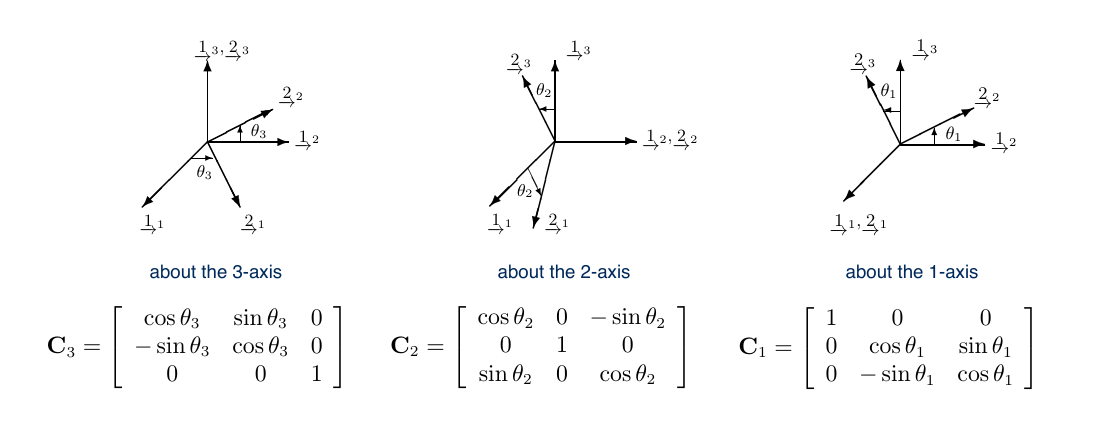
\includegraphics[scale=0.310]{img/coordinate_transforms/coordinate_rotations_4.jpeg}
\end{center}
\caption{Euler angles.}
\label{coordinate_rotations_4}
\end{figure}

Euler angles are attractive in part because they are
a parsimonious representation requiring only three parameters instead
of nine for a full rotation matrix. Unfortunately,
Euler angle representations are subject to what are
called singularities. Singularities complicate
state estimation because they represent particular rotations from which to
Euler angles are indistinguishable. Neither quaternions, see section \ref{unit_quaternion} nor
rotation matrices, section \ref{direction_cosine_matrix}, suffer from this problem at the expense
of using more parameters.

\subsection{Unit quaternion}
\label{unit_quaternion}

A second way to represent rotations is to use something called unit quaternions. Quaternions are an interesting
mathematical topic in their own right. However, it is sufficient to note that a unit quaternion can be represented as
a four-dimensional vector of unit length that parameterizes a rotation about an axis
defined by the vector $\mathbf{u}$, and an angle $\phi$ about that vector, see Figure \ref{coordinate_rotations_3}. 

\begin{figure}[!htb]
\begin{center}
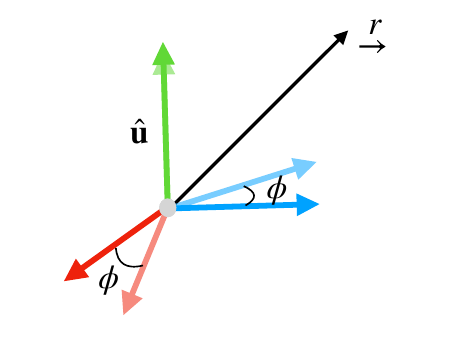
\includegraphics[scale=0.290]{img/coordinate_transforms/coordinate_rotations_3.jpeg}
\end{center}
\caption{The vector $\mathbf{u}$, and the angle $\phi$.}
\label{coordinate_rotations_3}
\end{figure}

Thus, we have the follwing equations

\begin{equation}
\mathbf{q} = 
\begin{bmatrix}
q_w \\
\mathbf{q}_{\nu}
\end{bmatrix} = 
\begin{bmatrix}
\cos(\frac{\phi}{2}) \\
\hat{\mathbf{u}}\sin(\frac{\phi}{2})
\end{bmatrix}, ~~ ||\mathbf{q}|| = 1
\end{equation}

We can convert a quaternion
to a rotation matrix by using the followin algebraic expression. 


\begin{equation}
\mathbf{r}_b = \mathbf{C}(\mathbf{q}_{ba})\mathbf{r}_a
\end{equation}

where 

\begin{equation}
\mathbf{C}(\mathbf{q}) = (q_{w}^2 - \mathbf{q}_{\nu}^T\mathbf{q}_{\nu})\mathbf{I} + 2\mathbf{q}_{\nu}\mathbf{q}_{\nu}^T + 2q_w[\mathbf{q}_{\nu}]_{\times}
\end{equation}

with

\begin{equation}
[\mathbf{a}]_{\times} =
\begin{bmatrix}
0 & -a_z & a_y \\
a_z & 0 & -a_x \\
-a_y & a_x & 0
\end{bmatrix}
\end{equation}

Quaternions have the advantage that they do not suffer from singularities and they only need
four parameters instead of nine in order to represent 3D rotations. 



Each represenation has advantages and disadvantages. A rotation matrix can
represent any rotation but requires nine parameters
and has six constraints. A unit quaternion can also be
used to represent any rotation, but it also has a constraint. To use a unit quaternion to
actually rotate a vector, we also require some additional algebra beyond simple matrix multiplication. Finally, Euler angles are unconstrained, intuitive to visualize and
use only three parameters, but are subject to singularities. Figure \ref{coordinate_rotations_5} summarizes the three approaches

\begin{figure}[!htb]
\begin{center}
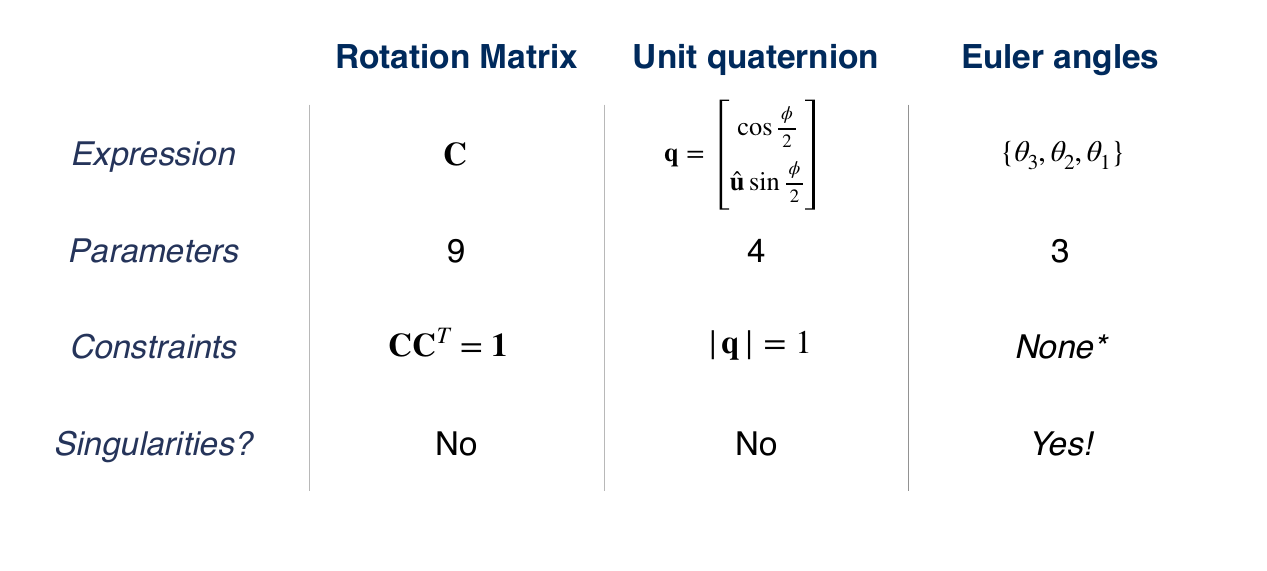
\includegraphics[scale=0.290]{img/coordinate_transforms/coordinate_rotations_5.jpeg}
\end{center}
\caption{Comparison of rotation representation approaches.}
\label{coordinate_rotations_5}
\end{figure}


To summarize, vector quantities can be expressed in different reference frames
through rotations and translations. Rotations can be parameterized
by rotation matrices, quaternions, or Euler angles, each of which has advantages
and disadvantages.
 
